\section*{Linear Regression in Practice}

\subsection*{Residual Analysis}

\textbf{Q.} How to check that the linear model is an appropriate model for the data? How to check equal variances? \\
~\\
In simple linear regression, the model assumes that
\begin{align*}
Y|x_i = \beta_0 + \beta_1 x_i + E_i
\end{align*}
and residuals can be used to approximate $E_i$, which are also random variables, are given by
\begin{align*}
\widehat{E}_i = Y|x_i - \widehat{Y|x_i} = \beta_0 + \beta_1 x_i + E_i - (B_0 + B_1 x_i),
\end{align*}
which follows a normal distribution. We can calculate the mean
\begin{align*}
\U{E}[\widehat{E}_i] & = \beta_0 + \beta_1 x_i + \U{E}\left[E_i - B_0 - B_1x_i \right] = 0,
\end{align*}
and variance
\begin{align*}
\U{Var}[\widehat{E}_i] & = \U{Var}\left[E_i - B_1 x_i - (\beta_0 + \beta_1 \overline{x} + \overline{E} - B_1 \overline{x}) \right] \\
& = \U{Var}\left[E_i - \overline{E} + B_1(\overline{x} - x_i) \right] \\
& = \U{Var}\left[E_i - \overline{E} + (\overline{x} - x_i)\cdot \left(\beta_1 + \frac{\sum(x_j-\overline{x})E_j}{S_{xx}} \right) \right] \\
& = \U{Var}\left[E_i - \overline{E} +  \frac{(\overline{x} - x_i)\sum(x_j-\overline{x})E_j}{S_{xx}} \right] \\
& = \sigma^2 + \frac{\sigma^2}{n} + \frac{(\overline{x}-x_i)^2\sigma^2}{S_{xx}} - 2\U{Cov}[E_i, \overline{E}] + 2\U{Cov}\left[E_i, \frac{(\overline{x} - x_i)\sum(x_j-\overline{x})E_j}{S_{xx}} \right] \\
&\qquad\qquad\qquad - 2\U{Cov}\left[\overline{E}, \frac{(\overline{x} - x_i)\sum(x_j-\overline{x})E_j}{S_{xx}} \right],
\end{align*}
where
\begin{align*}
\U{Cov}[E_i, \overline{E}] & = \frac{1}{n}\sum_{j=1}^n \U{Cov}[E_i, E_j] = \frac{1}{n}\sigma^2, \\
\U{Cov}\left[E_i, \frac{(\overline{x} - x_i)\sum(x_j-\overline{x})E_j}{S_{xx}} \right] & = (\overline{x} - x_i)\sum_{j=1}^n (x_j-\overline{x})\cdot \U{Cov}\left[E_i, \frac{E_j}{S_{xx}} \right] = -\frac{(\overline{x}-x_i)^2}{S_{xx}}\sigma^2, \\
\U{Cov}\left[\overline{E}, \frac{(\overline{x} - x_i)\sum(x_j-\overline{x})E_j}{S_{xx}} \right] & = \frac{\overline{x}-x_i}{n}\sum_{j=1}^n (x_j-\overline{x})\U{Cov}\left[E_j, \frac{E_j}{S_{xx}} \right] = \frac{(\overline{x} - x_i)\sigma^2}{nS_{xx}} \sum_{j=1}^n (x_j - \overline{x}) = 0.
\end{align*}
Therefore,
\begin{align*}
\U{Var}[\widehat{E}_i] = \U{Var}\left[Y|x_i - \widehat{Y|x_i} \right] = \left(1 - \frac{1}{n} - \frac{(x_i-\overline{x})^2}{S_{xx}} \right)\sigma^2.
\end{align*}
Note that this is different from the distribution of \underline{prediction}
\begin{align*}
\U{Var}[\widehat{Y|x} - Y|x] = \left(1 + \frac{1}{n} + \frac{(x-\overline{x})^2}{S_{xx}} \right)\sigma^2,
\end{align*}
where in prediction, we are not choosing $x$ to be equal to any of the $x_1, \ldots, x_n$ that are used to estimate $\beta_1$ and $\beta_0$. When we assume that $x_i$ is among those we use for estimation, there are additional covariance terms.

Therefore, if we plot the residuals, we can see when the point $x_i$ is far from mean $\overline{x}$, the variance is smaller. In addition, the points should uniformly reside above the line $y = 0$ and below this line. This can be used to check for equal variance and linearity of our model. For instance, the following shows a residual plot with problems.

\begin{figure}[H]
	\centering
	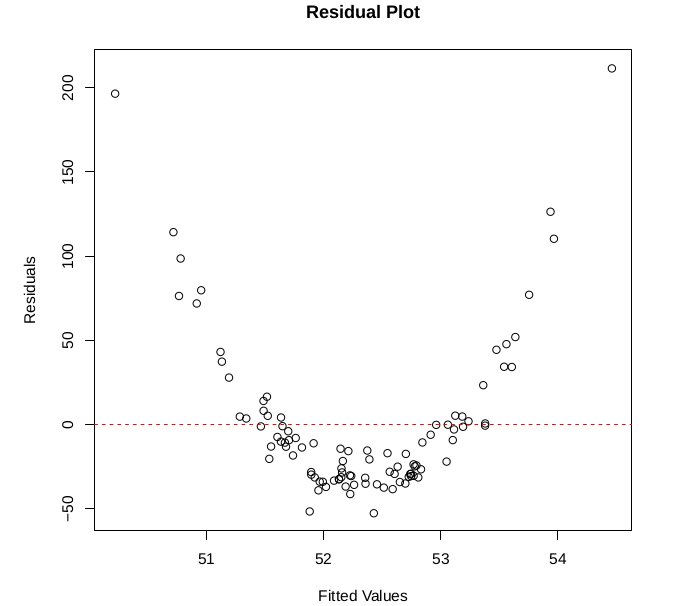
\includegraphics[width=12cm]{./images/s7fig1.png}
\end{figure}


\subsection*{Linear Regression using R}

In addition to Mathematica we use in the lecture, R is widely used for studies of data analysis. Here is an example of using R to perform a simple linear regression.

\begin{figure}[H]
	\centering
	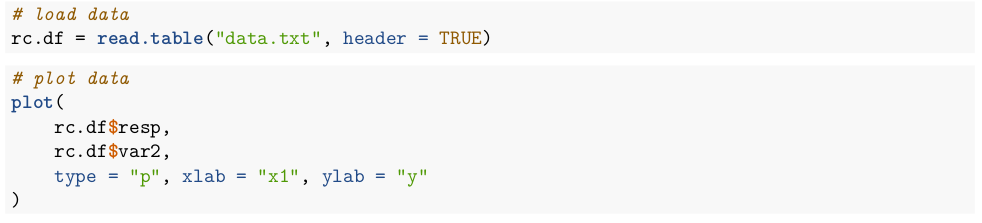
\includegraphics[width=\linewidth]{./images/s7fig4.png}
\end{figure}
\begin{figure}[H]
	\centering
	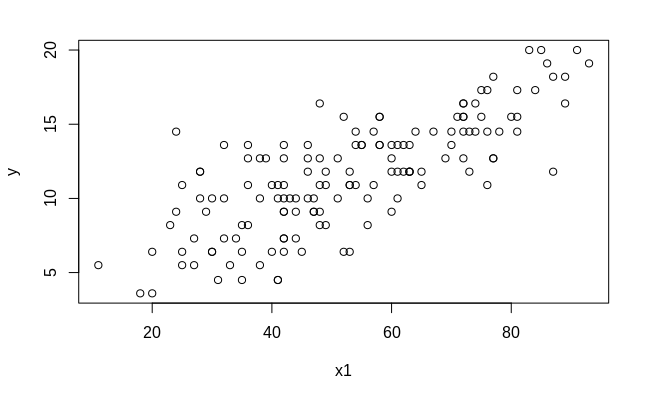
\includegraphics[width=12cm]{./images/s7fig5.png}
\end{figure}
\begin{figure}[H]
	\centering
	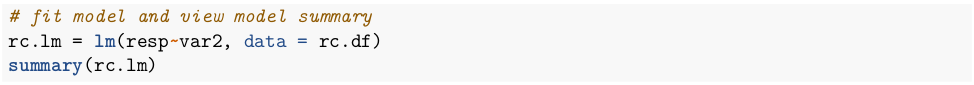
\includegraphics[width=\linewidth]{./images/s7fig6.png}
\end{figure}
\begin{figure}[H]
	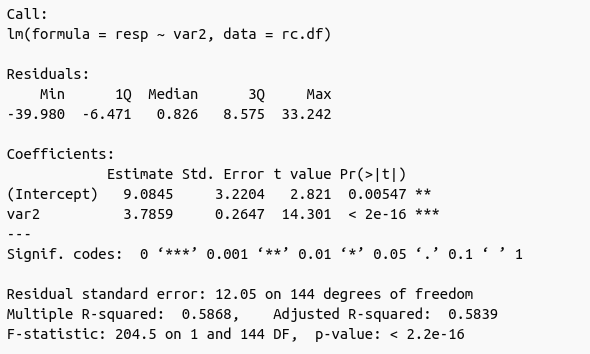
\includegraphics[width=12cm]{./images/s7fig2.png}
\end{figure}
\begin{figure}[H]
	\centering
	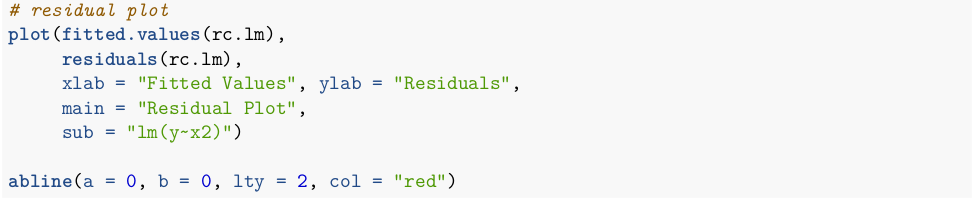
\includegraphics[width=\linewidth]{./images/s7fig7.png}
\end{figure}
\begin{figure}[H]
	\centering
	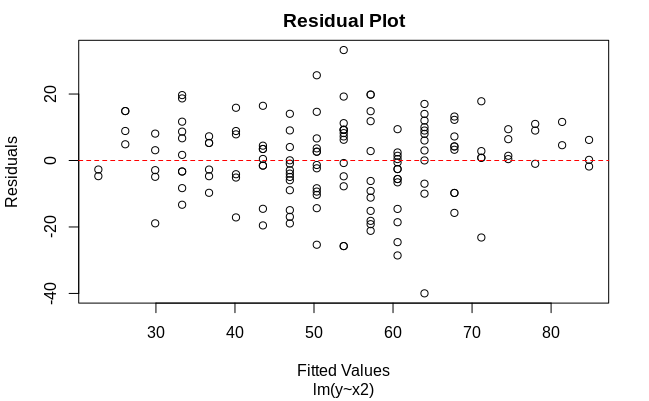
\includegraphics[width=12cm]{./images/s7fig3.png}
\end{figure}

